\documentclass[11pt, oneside]{article} 
\usepackage{geometry}
\geometry{letterpaper} 
\usepackage{graphicx}
	
\usepackage{amssymb}
\usepackage{amsmath}
\usepackage{parskip}
\usepackage{color}
\usepackage{hyperref}

\graphicspath{{/Users/telliott_admin/Dropbox/Tex/png/}}
% \begin{center} 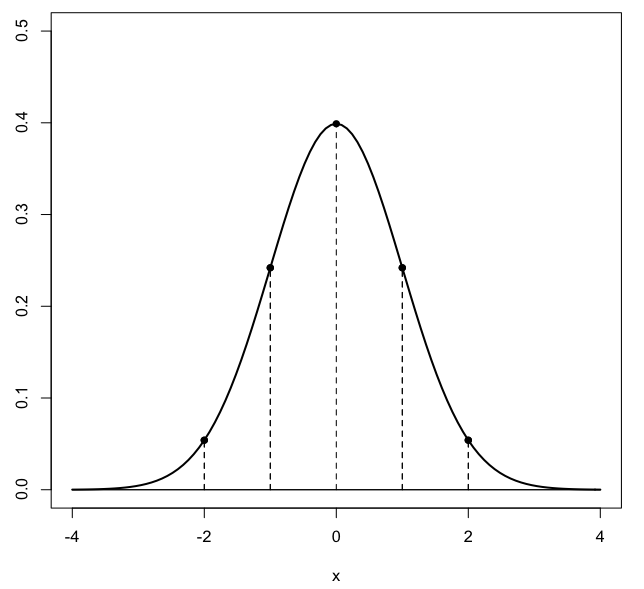
\includegraphics [scale=0.4] {gauss3.png} \end{center}

\title{Numbers}
\date{}

\begin{document}
\maketitle
\Large
Our ideas about sets of numbers start with the counting numbers or positive integers
\[ \mathbb{N} = 1, 2, 3 \dots \]
which is an infinite set.  

Proof by contradiction:  assume there is a greatest natural number.  Add $1$ to it.  $\square$

We extend $\mathbb{N}$ by adding the number or additive identity $0$, plus the negatives of all the numbers in $\mathbb{N}$:
\[ \mathbb{Z} = \{ \dots - 3, -2, -1 , 0 , 1, 2, 3 \dots \} \]

$\mathbb{Z}$ is what they call a \emph{ring}.  The standard operations like addition and multiplication are defined and allowed but not division. 

Then we say, we want division.  We get
\[ \mathbb{Q} = \frac{p}{q}, \ \ \ \  p \in \mathbb{Z}, q \in \mathbb{N} \]

Now, the rational numbers $\mathbb{Q}$ have great properties.  In particular, for any two rational numbers one can find another such number which lies between them:
\[ r = \frac{1}{2} \ [ \ \frac{p_1}{q_1} +  \frac{p_2}{q_2} \ ] \]
This is a rational number and it lies between the two numbers we started with.

\[ \frac{1}{2} \ [ \ \frac{p_1}{q_1} +  \frac{p_1}{q_1} \ ] \ < r < \ \frac{1}{2} \ [ \ \frac{p_2}{q_2} +  \frac{p_2}{q_2} \ ] \]

So it is not unreasonable to have the idea that the number line can be divided into pieces as small as you like by finding rational numbers between rational numbers between rational numbers, and so on.

It sounds good, but there are some problems.

First, some numbers cannot be expressed in this way but are \emph{irrational}.  For example:  $\sqrt{2}$, $\sqrt{3}$, $\sqrt{5}$, $\sqrt{7}$, etc..  And don't forget $\pi$ and $e$.

This lead Dedekind to formulate the famous Dedekind cut.  Visualize the standard number line as an infinite line on a piece of paper.  

\begin{center} 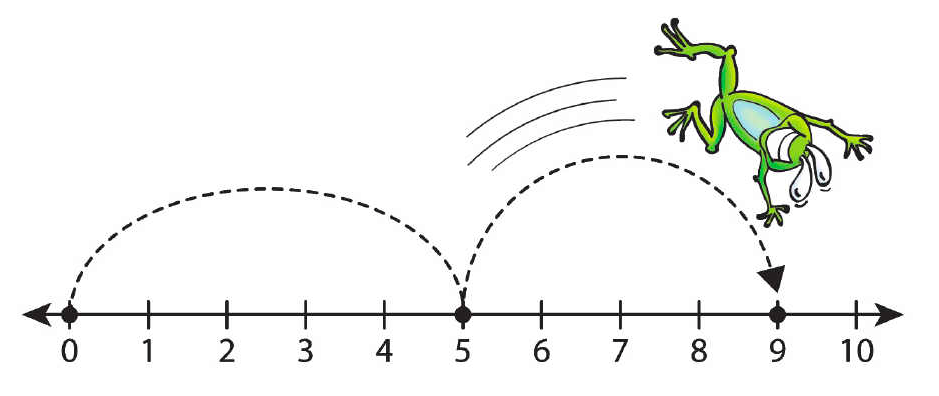
\includegraphics [scale=0.4] {number_line.png} \end{center}

Each number corresponds to a cut, a knife-edge coming down on this number line.  Every other number is either $>$ or $<$ the number specified by the cut.

One position is $\sqrt{2}$, one is $7/4$ and so on. So then for any given cut there are three possibilities:  

( i) the cut is at a rational number $p/q$ and that number is the smallest number of the set of numbers $\ge p/q$.

(ii) the cut is at a rational number $p/q$ and that number is the largest number of the set of numbers $\le p/q$.

(iii) the cut is at an irrational number $r$ and the sets above and below \emph{do not have a smallest or largest number} that is in the set.  The number at the cut is the only bound that we can specify.

That is actually OK.

I can live with what we've said so far.  Here's what's really weird.  Cantor proved that the set $\mathbb{Q}$ is \emph{countably finite}.  Each element in $\mathbb{Q}$ can be paired in order with a member of $\mathbb{N}$.

But the real numbers, $\mathbb{R}$, are countably infinite.  So in some sense, there are many, many, many more irrational numbers than rational numbers.

So when we say that the set of numbers $r < 1$ has \emph{no greatest element}, our problem is two-fold.  We can pick a large rational member of $r < 1$, but we can always find a larger rational element.  

And once we get really close with the large rational element, there are infiinitely more irrational than rational ones waiting beyond.  And yet, given any such very close irrational number, we can always find a larger rational number less than the bound.

I told you it was weird.

\end{document}